\documentclass[10pt,norsk,a4paper]{article}
\usepackage[utf8]{inputenc}
\usepackage[T1]{fontenc}
\usepackage[norsk]{babel}
% - PDF-relatert
\usepackage{hyperref,pdfpages,hypcap}
\hypersetup{colorlinks=true,allcolors=.}
\newcommand\fhref[2]{%
	\href{#1}{#2}\footnote{\url{#1}}%
}
% Andre pakker
\usepackage[cm]{fullpage}
\usepackage{parskip,multicol,textcomp,amssymb,graphicx,color,enumitem,cleveref}
% - Korreksjon av fotnoter i seksjoner/overskrifter
\usepackage[stable]{footmisc}
% - Skrifttype
\usepackage[bitstream-charter]{mathdesign}
% - Kommentarer
\usepackage{comment}
\usepackage{epstopdf}

\epstopdfsetup{outdir=./}


\title{Generalforsamling \\
	Våren 2019\\[3cm]
	
\includegraphics[width=0.5\textwidth]{cyb-logo.eps}\\[-.5cm]}
\date{23.\ mai 2019}
\author{Cybernetisk Selskab}

% Blank header, samt footer med side x av y
\usepackage{fancyhdr}
\pagestyle{fancy}
\renewcommand{\headrulewidth}{0pt}
\fancyhead{}
\cfoot{Side~\thepage\ av~\pageref*{lastpage}}


\begin{document}

\maketitle{}
\newpage
\tableofcontents

\section{Valg av møteleder}
Andreas Nyborg Hansen velges ved akklamasjon.

\section{Valg av referent}
Lee Kvåle velges ved akklamasjon.

\section{Valg av protokollunderskrivere}
Trine Høyås og Marie Reichelt velges ved akklamasjon.

\section{Valg av tellekorps}
Adrian Helle og Hilmar Elverhøy velges ved akklamasjon. 

\section{Godkjenning av innkalling}
Godkjennes ved akklamasjon.

\section{Godkjenning av dagsorden}
Godkjennes ved akklamasjon.

\newpage

\section{Semesterberetninger}
\subsection{Semesterberetning ved leder}

Hei til deg, CYB-er og bidragsyter,

\begin{multicols}{2}

``Takk for at du er her.'' Slik lød starten på høstens
generalforsamling, og lite visste man om utfordringene som kom til å
treffe interne på tvers av grupper og spesielt på tvers av synspunkter.
I motsetning til forrige generalforsamling har vi færre og mindre
kontroversielle endringsforslag lagt fram, og nettopp burde disse timene
faktisk bli litt kortere enn de var i høst. Velkommen!

Som i fjor høst, har vi hatt henholdsvis 25\% og 15\% flere interne på
våren enn i 2018 og 2017. Totalt har de bidratt med ca. 150 flere
interntimer sammenlignet med i fjor og nesten like mange timer som i
2017. De har bidratt gjennomsnittlig 11,8 timer hver, i motsetning til
13,6 og 14 timer i 2018 og 2017. Nok en gang er tallene basert rent på
hva som er registrert av bongført aktivitet. Om man utelukker alle
timene med ikke-bongførte bidrag er det en fortsatt positiv trend som
jeg håper fortsetter.


Mangfoldet i interne skylder stor takk til gruppeledere som har aktivt
rekruttert og fått inn nye frivillige. Som deltaker på
generalforsamlingen er du forhåpentligvis en av 612 registrerte
medlemmer. Antallet har derimot sunket med henholdsvis 7,6\% og 2,2\%
sammenlignet med toppvåren 2018 på 663 og våren 2017 med 626.


Dette semesteret har arrangementsgruppa planlagt og gjennomført, i lag
med PR og blæst fra promoteringsgruppa, i overkant av 30 arrangementer.
Mye variert liv og røre. Torsdagsklubben ble til torsdagspub, og blander
drinker med forskjellige tema. Med februar kom 50-årsfeiringen av
foreningen. Hvem er her om 50 år? Igjen har vi, nå for tredje semester
på rad, gjennomført en fellesfest for de interne med Realistforeningen,
denne gangen i RF-kjelleren. Det er bare noen veldig få av en haug med
arrangementer. Alle bidragene til festene, feiringen, arrangementene,
reale temafester og mer til, fortjener en stor takk: dere bringer et
festlig avbrekk i hverdagen, utover kaffe, øl og sprit.


I fjor fikk vi inn solide endringer til vedtektene, og fikk tatt en
diskusjon som andre studentkjellere har måttet ta i etterkant av
universitetets nye retningslinjer mot trakassering. Det krevde mye fra
både interne og medlemmer i foreningen. Veien har fortsatt fremover, og
med både retningslinjer for medlemmer og styremedlemmer har vi
verktøyene. Spørsmålet fremover er hvorvidt vi kan fortsette å anvende
disse på en god måte.


Mange prosjekter har vært påbegynt, mens desto færre er avsluttet.
Gruppeautonomi har ikke endret seg mye, i motsetning til en
onboardingsprosess for nye interne som har fått litt mer kjærlighet i
form av ny.cyb.no. Ny espressomaskin og pengene til dette jobbes
fortsatt med. Et bedre definert forhold med foreningene er utarbeidet,
som vi må få innspill på, og styrkes fortsatt av god kommunikasjon og
samarbeid med linjeforeningene. Eksempelvis er festen i morgen et godt
eksempel på hva man kan få til når linjeforeninger føler et eierskap og
tilhørlighet til Escape og CYB.

Endelig har vi en kjelleravtale som kan sees med det blotte øyet, og i
verste fall med en enkel kikkert. Ny avtale medfører noen endringer, men
arbeidet fortsetter med å redusere hvordan disse påvirker oss.


Utfordringene fremover er av forskjellig art. Opprydding i et regnskap
og en ny kjelleravtale kan være komplisert, men opprydding i
organisasjonskultur er komplekst. Kompleksitet i organisasjoner, som
kompleksitet i store informasjonssystemer, tar tid å endre på, og det er
ingen enkel måte å bryte ting ned i uavhengige biter. Når friksjon
oppstår internt, enten det er mellom grupper, styrer eller individer, må
vi finne løsningene som reduserer friksjonen. Internt er man ikke en
eneste stor og alltid samlet gjeng. Respekten for hverandre og tiden vi
dedikerer til foreningen må fortsatt komme først. Selv når vi er uenige
innad står vi samlet utad.

Jeg vil utrette en personlig takk til alle kaféfunksjonærene, de få
barfunksjonærene, utlånsarbeiderne, styremedlemmene i kjeller- og
hovedstyrene og interne jeg har vært med siden 2015.

For meg er det ingen tvil om at tiden i CYB har gitt mye. Venner, gode
stunder, utfordringer, Eurovision (en helt egen stund), samboer,
drikkepress, påfølgende lærdom dagen derpå, og mer til. Ingen av oss er
perfekte, men sammen har man utgjort et lite mikrosamfunn som jeg på
ingen måte kan si at jeg angrer på. Jeg er takknemlig for de styrene før
min tid, styrene i 2017-2018, styrene på høsten, og styrene denne våren,
og spesielt alle de interne som har bidratt med deres tid og energi. Alt
det nye blodet foreningen har fått. Uten de ville vi ikke ha kommet så
langt som vi har. Uten nye bidrag kommer vi ikke lengre.
\end{multicols}

Som i fjor høst, og for siste gang, ``takk for at du er her'', og ``vi
har mye å se frem til''.

\textbf{Thor K. Høgås}, \\
avtroppende leder, \date{\emph{23. mai 2019}}

\newpage

\subsection{Semesterberetning ved kjellermogul}

\begin{multicols}{2}
Året startet med CYB50, som hadde vært planlagt i lang tid. Mandagen startet
med lansering av fjerde utgave av Ifis eget tidsskrift, Output, etterfulgt av
konsert. Oppmøtet var ikke så godt som håpet på, men de som møtte opp så ut
til å kose seg. På tirsdagen hadde vi åpen kosetirsdag med pizza og representasjon
av arbeidsgruppene i CYB. Her var oppmøtet ganske godt, slik det pleier å være
når man serverer pizza her på bygget. Fredagen gikk på skinner med godt oppmøte
og god feststemning. Dette var en god måte å starte helgen på og å varme opp til
gallaen på lørdagen. Vi serverte også øl som vi hadde vært med og brygget hos Aass.
Dette solgte veldig godt, og de 1000 literne vi brygget har nesten blitt
drukket opp allerede.

Baren har hatt en liten revolusjon dette semesteret. Det er mange nye
barfunksjonærer og flere nye skjenkemestere. Vi har dette semesteret
oppdatert drinkmenyene og laget flere forskjellige menyer. Nå har vi
både meny for drinker under 22% og meny for mocktails i tillegg til
flere versjoner av den vanlige drinkmenyen kategorisert på forskjellige
måter. Nytt av året har vi nesten fast servert drinker (under 22%) på
fredagspuber. Dette har vært en stor suksess og har blitt godt tatt imot
av gjester. Det har også ført til en større profitt på fredagspuber.

På Ettermiddagen i år hadde vi ikke værgudene på vår side med snøstorm
og fint vær om hverandre. Trenden om at vi kun har utebar denne dagen
annethvert år stemte nok en gang. Denne gangen droppet vi derimot ikke
å ha to barer, men prøvde oss heller på et helt nytt konsept: To barer
i Escape! Den ekstra baren sto i hjørnet foran DJ-bua. Her ble det
servert drinker, ølet som ble brygget til CYB50 og cider. Dette fungerte
veldig greit siden DJ sto oppe på scenen og derfor ikke ble gjemt bort bak
masse utstyr. Selv uten pils på tapp da slangen begynte å lekke halvveis
utpå kvelden, ble Ettermiddagen en stor suksess!

SALUTT-kurs har vært et stort tema både dette semesteret og forrige.
Det var satt opp to kurs spesifikt for studentpuber i januar hvor vi
hadde mange av våre funksjonære som deltok. Vi har ennå ikke måtte
stenge tidlig grunnet manglende SALUTT-kurs dette semesteret.
Forhåpentligvis slipper vi dette fremover også.

Dette semesteret har vi jobbet med å få en mer tydelig musikkprofil i Escape.
Vi har hatt et ønske om å ikke lenger promotere oss som en brun pub, men
heller et sted for alle forskjellige studenter. Vi har mange gjester som er
glade i å danse, og derfor har vi gått mer over til å spille musikk som er
lett å like for de fleste og også som det er mulig å danse til. Vi har også
fått mange nye flinke DJ-er dette semesteret som både spiller hos oss
og på andre utesteder.

Det tekniske holder vi også på å overhale. Porten er omsider blitt fikset,
og vi har på nytt tilegnet oss kunnskapen om at vi har mulighet til å styre
persiennene så lenge det ikke er «storm» oppe i 10. etasje. Nytt av året
har vi ikke lenger lov til å ha ytterdøra til lokalet stående oppe siden
dette visstnok kan føre til frost i et rør og skadedyr, som om vi ikke allerede
har nok med sølvrke. Etter en opphetet og lang diskusjon med EA kom man frem
til at døra skulle stå lukket men ulåst. Dette har heldigvis ikke resultert i
færre besøkende, men vi har hatt problemer med å låse døra igjen etter
klokka 3.00 om natta.

Arrangementskoordinator har vært et verv som har vært vanskelig å definere.
Vi har sett at arbeidsoppgavene for det meste omhandler spritbar og store
arrangementer der det er nødvendig å ha et ekstra styremedlem for å få alt
til å gå i hop. Arbeidsoppgavene til dette vervet har dette semesteret blitt
bedre definert og vervbeskrivelsen har blitt forandret henholdsvis.

Kjellerstyrets internfest dette semesteret ble en skikkelig vikingfest!
Lokalet var dekorert med skjold og vikingskip i god stil. Nikolas og faren
disket opp med helstekt lam, og vi serverte mjød. Den nyoppfunnede leken
«klosster» ble en stor suksess og resulterte i at prosjektoren ble slått ut
av posisjon og bukser ble revet opp. Alt i alt virket det som at
folk var veldig fornøyde.

Forrige helg ble det både arrangert 17. mai og nostrabrunch i Escape.
På 17. mai ble det servert snitter og kaker, og det var mange til stede
som ikke hadde feiret 17. mai her før. Nostrabrunchen ble arrangert sammen
med Placebo. Dette var en suksess, og dagen ble avsluttet med visning av Eurovision.

Fremover har vi mye å glede oss til. Like rundt hjørnet er det en fest arrangert
av linjeforeningene på bygget, nok en temafest og så er det semestersluttfest.
Vi har også julitrefest i sommer for alle interne, både nye og gamle, denne
gangen muligens med servering. Det er også viktig å huske at det ikke er så
fryktelig lenge til en ny studiestartuke. I år har vi som tidligere, men nå
også på papiret, ansvar for gaffateipfesten og ctrl+alt+del.

Jeg vil til slutt takke kjellerstyret for et veldig godt gjennomført semester,
og de interne som står på dag og natt for at foreningen skal fortsette å
gå så godt som den gjør.
\end{multicols}
\textbf{Marie Reichelt}, \\
kjellermogul, \date{\emph{23. mai 2019}}

\newpage

\section{Kasserer orienterer}
Verken budsjettet eller regnskapet skal godkjennes da
de ikke er i en tilstand som behandles under generalforsamlingen.

Kasserer forklarer bakgrunnen for nåværende økonomiske vansker i foreningen, inkl. problemer med kassa. I løpet av året har kasserer jobbet på spreng for å føre momsrapporter og bilag, samt jobbet med å få oversikt over unødvendige utgifter sammen med leder. Lærdommen er at man ikke kan bytte ut kritiske komponenter uten tilstrekkelig testing, og at det er nødvendig med prosjektpersoner som kan jobbe med slike ting når det skjer.

Videre vil CYB velge tre ``økonomimestre'' med tre forskjellige fokusområder
\begin{itemize} 
	\item Oppgjørsmester
	\item Småkjøpsmester
	\item Fakturamester
\end{itemize}

Vi vil også innhente en regnskapsfører for å hjelpe oss med å få styr på ting, samt ha regelmessige økonomimøter og økonomikurs.

Vi må få til et revisjonsutvalg og vi burde bytte bank.

Tor-Aksel Solberg trekker seg offisielt som kasserer. Vervet vil etterfylles av hovedstyret.

\subsection{Spørsmålsrunde}
\emph{Hvordan skal man insentivisere til å ta økonomimesterposisjonene?}

F.eks. nostrabevis for de som ikke nødvendigvis vil være i styret, men vil ha mulighet til å delta på nostraarrangement. 

\emph{Hva er Nostra, for de som ikke vet?}

Nostra er samarbeidsorgan mellom kjellerpubene.

\emph{Hvordan skal man fylle mesterrollene?}

Vi må i alle fall få dem inn i Altinn så de får tilganger til ting. Stillingene kan fylles på GF eller av HS.

\emph{Det virker ikke nødvendigvis helt bra å gi folk tilganger til kontoene om de ikke er i styret.}

Om vi bytter bank kan vi gi begrensede tilganger som vil tjene formålet uten videre risiko. Om HS mener at økonomimestrene er tillitsverdige burde det være godt nok ettersom HS har ansvar for kontoene.

\section{Kontigentfastsettelse}
Hovedstyret foreslår å holde medlemskontigenten på kr.~40,-.
\subsection{Informasjon}
Hovedstyret anbefaler at det neste styret setter kontigenten opp til 50kr for å kunne søke Frifond fra 1. januar 2020.
\subsection{Bestemmelse}
Medlemskontigenten på 40kr godkjennes ved akklamasjon.

\newpage

\section{Valg}

\begin{minipage}[t]{0.49\textwidth}
\subsection{Hovedstyret}
Man velges inn i hovedstyret for ett år av gangen.

\subsubsection{Leder}
\textit{Leder presenterer vervet.}

Fredrik Magnussen stiller som leder. 

\emph{Hvordan ønsker du å forbedre forhold mellom HS og KS?}

Faste møter, bedre oppmøte på kosetirsdag, bedre kommunikasjon, bedre synlighet.

\textit{Fredrik Magnussen velges ved akklamasjon.}
\subsubsection{Nestleder}
\textit{Nestleder presenterer vervet.}

Martin Heggem stiller som nestleder.

\emph{Har du planer om å fikse internkort for andre foreninger?}

Det burde være overkommelig. 

\emph{Kommer du til å fikse livstidskort?}

Har veldig lyst på ett selv så forhåpentligvis.

\textit{Martin Heggem velges ved akklamasjon.}
\subsubsection{Arrangementssjef}
\textit{Arrangementssjef presenterer vervet.}

Åsmund Rosendahl stiller til arrangementssjef. 

\emph{Har du tenkt å ta opplæring i bongføring for arrmestre og funker?}

Det er nødvendig. 

\emph{Dersom en nyere intern vil ha vervet, vil du trekke deg?}

Dersom de ønsker vervet, ja. 

\textit{Åsmund Rosendahl velges ved akklamasjon.}
\subsubsection{Rekrutteringsansvarlig}
\textit{Leder presenterer vervet.}

Nelin Gökbel stiller som rekrutteringsansvarlig.

\emph{Will you try to make people communicate more in English on Slack/other channels?}

Yes, that is the goal.

\textit{Nelin Gökbel velges ved akklamasjon.}
\subsubsection{Internansvarlig}
\textit{Internansvarlig presenterer vervet.}

Markus Høydalsvik og Saira Hussain stiller, via Thor Høgås og Isak Fyksen, respektivt. 

\emph{Markus was here earlier, why is he not here now?}

He has an exam tomorrow morning, and could not be here.

\emph{Can Saira also use Cupid's bow and arrow?}

Unknown.

\textit{Markus Høydalsvik blir valgt som internansvarlig.}
\end{minipage}
\begin{minipage}[t]{0.49\textwidth}
\subsection{Kjellerstyret} %TODO Oppdater listen med verv
Alle verv som er til valg i kjellerstyret gjelder for ett semester av gangen. Med unntak av Økonomiansvarlig som blir valgt inn for to semester.

\subsubsection{Innkjøpsansvarlig}
\textit{Innkjøpsansvarlig presenterer vervet.}

Nikolas Hemer Martin stiller som innkjøpsansvarlig. 

\emph{Hvordan har du tenkt å opprettholde utvalget mtp. økonomisituasjonen?}

Kommunisere godt med økonomigruppa, er selv innvolvert der. Satser på god erfaringsoverføring fra tidligere innkjøpsansvarlig. 

\emph{Du har andre styreverv og jobb, hvordan skal du balansere dette med styreverv?}

Har avspasering og har satt av mer tid generelt, så det burde gå bra.

\emph{Hvordan vil du forholde deg til at det vi har på lager er verdi vi sitter inne med, så vi ikke ender opp med å miste penger fordi vi bestiller nye ting?}

Må lære fra tidligere innkjøpsansvarlig hvordan vurdere det. 

\emph{Du har planer om å reise bort i sommer. Hvordan skal du koordinere innkjøp for fadderuka mtp. dette?}

Må sette opp en plan, helst med tidligere innkjøpsansvarlig sin hjelp.

\emph{Har du noen tanker om hvordan du skal inngå avtaler med leverandører for å få gode priser?}

Må be om hjelp og råd fra andre, dette er en del av erfaringsoverføringen. 

\emph{Ang. ferieopphold, det burde gå an å gjøre bestillinger fra utlandet også.}

Er interessert i å delegere arbeid uansett, har en liten gruppe tilgjengelig som kan hjelpe med innkjøp.

\emph{Hva tenker du å gjøre når du har to roller på dagen@ifi?}

Føler de er litt separate, som innkjøpsansvarlig skal arbeidet være forberedende, samme med arbeidet som fagansvarlig. Det burde derfor ikke krasje. 

\emph{Tidligere har kafésjef hatt ansvar for bestillinger for kaféen?}

Det kommer an på om neste kafésjef har kapasitet til å ta det.

\textit{Nikolas Martin velges ved akklamasjon.}
\subsubsection{Barsjef}
\textit{Barsjef presenterer vervet.}

Isak Fyksen stiller til gjenvalg.

\emph{Ingen spørsmål.}

\textit{Isak Fyksen blir valgt ved akklamasjon.}
\subsubsection{Kafésjef}
\textit{Kafésjef presenterer valget}

Kine Grøtt stiller som kafésjef via Trine Høyås.

\emph{Syns Kine kaffen vår er bedre enn kaffen på Espresso House?}

Ja.

\textit{Kine Grøtt blir valgt ved akklamasjon.}
\subsubsection{Teknisk ansvarlig}
\textit{Teknisk ansvarlig presenterer vervet.}

Jørgen Spilling stiller til gjenvalg.

\emph{Hvilke oppgraderinger o.l. har du planlagt for neste semester?}

Vil gjerne få flere mikrofoner. Ellers er det ingenting planlagt. 

\textit{Jørgen Spilling blir gjenvalgt ved akklamasjon.}
\subsubsection{DJ-sjef}
\textit{Kjellermogul presenterer vervet.}

Hanna Nikoline Støen stiller via Anja Gjerpe.

\emph{Har Hanna noen tanker om musikkprofilen til Escape?}

Vi kan regne med at hun gjerne vil ha musikk som folk liker så folk vil komme på festene våre.

\emph{Kommer musikkprofilen vår til å forholde seg noenlunde profesjonell?}

Utad, ja. På interne arr, tvilsomt.

\textit{Hanna Nikoline Støen blir valgt ved akklamasjon.}
\subsubsection{Utlånsansvarlig}
\textit{Utlånsansvarlig presenterer vervet.}

Bendik Berg stiller til utlånsansvarlig.

\emph{Ingen spørsmål.}

\textit{Bendig Berg velges ved akklamasjon.}
\subsubsection{Arrangementskoordinator}
\textit{Arrangementskoordinator presenterer vervet.}

Anja Gjerpe stiller til gjenvalg.

\emph{Hva er planene mtp. spritbar?}

Vil fortsette å utvikle menyer o.l.

\emph{Planer for alkoholfrie muligheter?}

Vil fokusere på alkoholfrie arr og fortsette å utvikle alkoholfri meny.

\emph{Skal vi bevege oss bort fra nittitallsdrinkene?}

Målet er å utvikle Escape-spesifikke drinker.

\textit{Anja Gjerpe velges ved akklamasjon.}

\end{minipage}

\newpage

\section{Vedtektsforslag}

\subsection{Personlig oppmøte eller mulighet for fullmakt}

Det foreslås at det først stemmes over hvorvidt man skal behandle \cref{sec:no-full} eller \cref{sec:full}. 

\begin{enumerate}
	\item Dersom \cref{sec:no-full} velges, stemmes det over.
		\begin{itemize}
			\item Går deretter videre til \cref{item:vote}.
		\end{itemize}
	\item Dersom \cref{sec:full} velges, stemmes det over.
		\begin{itemize}
			\item Dersom \cref{sec:full} vedtas, stemmer man over \cref{sec:begrenset_full} om begrensning i fullmaktssaker.
			\item Går deretter videre til \cref{item:vote}.
		\end{itemize}
	\item Det stemmes over \cref{sec:avstemning} om tydeliggjøring rundt skriftlig avstemning.\label{item:vote}
\end{enumerate}

\subsubsection{Alt. 1: personlig oppmøte kreves for å kunne avgi enhver stemme:
               nytt punkt under §7 eller tillegg til punkt §7g\label{sec:no-full}}
\begin{quote}
	Forslaget eliminerer muligheten for å avgi fullmakt til en annen person for å stemme.\\
	--- \emph{Nikolas Papaioannou}
\end{quote}

Hovedstyret \emph{støtter ikke} dette endringsforslaget.

Det foreligger \emph{to forskjellige implementasjonsforslag} for samme ordlyd.

\textbf{Alt. 1: nytt punkt under §7}
\begin{quote}
	\begin{enumerate}
		\item[§7k] Man må være personlig oppmøtt på generalforsamlingen for å kunne avgi stemme.
	\end{enumerate}
\end{quote}

\textbf{Alt. 2: endring av §7g}
\begin{quote}
    \begin{enumerate}
        \item[§7g] Stemmerett har alle som er medlem, jf. §2, minst én uke før generalforsamling,
                  \textcolor{green}{og som personlig møter opp på generalforsamling}.
    \end{enumerate}
\end{quote}

\subsubsection{Alt. 2.1: opptil én fullmakt kan avgis per person: to nye punkter under §7\label{sec:full}}

\begin{quote}
	Forslaget fastsetter muligheten og kravene for å avgi stemmer via fullmakt,
	og begrenser det til én fullmakt per hver stemmeberettigede til stede.
	Åpne for at hver oppmøtte kan maksimalt ha en fullmakt fra en annen person.
	Dette gjør at hvis man faktisk har en grunn til å ikke komme er det enda mulig å fikse med noe.\\
	--- \emph{Nikolas Papaioannou}
\end{quote}

Hovedstyret \emph{støtter} dette endringsforslaget.

\textbf{Nytt punkt under §7}


\begin{quote}
    \begin{enumerate}
        \item[§7k]
            Hver stemmeberettigede tilstede på generalforsamling kan stille med
            stemmefullmakt for én annen stemmeberettiget.

            Fullmakten må inneholde følgene punkter:
            \begin{itemize}
                \item Navn på hvem fullmakten er gitt til
                \item Navn på den som gir fullmakten
                \item Dato for generalforsamling
                \item Signaturer fra begge parter involvert
            \end{itemize}
    \end{enumerate}
\end{quote}

\subsubsection{Alt. 2.2: begrensning av fullmaktsmulighet\label{sec:begrenset_full}}
\begin{quote}
	Enda ett punkt som kan følge hvis punkt over går gjennom:\\
	--- \emph{Nikolas Papaioannou}
\end{quote}
Hovedstyret \emph{støtter ikke} dette endringsforslaget.

\textbf{Nytt punkt under §7}
\begin{quote}
    \begin{enumerate}
        \item[§7l] Fullmakter gjelder kun ved vedtektssaker og ikke valg av styremedlemmer.
    \end{enumerate}
\end{quote}

\textit{Vervet presenteres av Nikolas Papaiannou.}

\subsubsection{Spørsmål}
\emph{Hvordan er dette med fullmakter tenkt ang. å stille via andre?}

Ikke relevant, dette er kun tiltenkt for stemmesituasjoner.

\subsubsection{Diskusjon}
\begin{itemize}
	\item Forslag til redaksjonell endring, fullt navn i stedet for bare navn.
	\item Det er gode forutsigbare grunner til å være borte.
	\item Leder presenterer hovedstyrets syn på forslagene.
	\item Det er bra å spesifisere at fullmakten skal begrenses til en fullmakt per pers.
	\item Ang. sammenligningen med borettslag o.l., det kan kanskje være ønskelig å åpne for at personer som ikke er stemmeberettigede kan ha fullmakt på vegne av andre. 
	\item Det burde tydeliggjøres i vedtektsendringen at det ikke gjelder for oppløsning av CYB.
	\item Å formalisere fullmaktsprosessen hever terskelen for å delta i stemmesituasjoner via andre, så kun de som faktisk er dedikerte til foreningen og sakene vil mest sannsynlig gidde å gjøre det. 
	\item Vi er allerede i fare for å bli kuppet fordi vi gir stemmerett til alle som kommer inn i bartid.
\end{itemize}	

\emph{Angående tillegg på alternativ 2}
\begin{itemize}
	\item Dersom du gir fullmakten din til noen stoler du forhåpentligvis nok på dem til at de kan stemme over styremedlemmer også.
	\item Det burde være rom for å kunne spesifisere hvilke kandidater man evt. vil stemme på dersom man vet hvem som skal stille. 
	\item Dersom du er bekymret for at en person skal misbruke fullmakten du har gitt dem, ikke gi dem fullmakt!
	\item Det er sketchy å gi fullmakt til å velge styremedlemmer selv om du vet om en som skal stille. Tenk om kandidaten du ville stemme på ikke er forberedt?
	\item Dersom du som fullmaktholder ikke følger det som står i fullmakten din bør du ikke ha den i utgangspunktet.
\end{itemize}
	
\subsubsection{Bestemmelser}
\emph{Valg mellom alternativ 1 og 2.}

Alternativ 2 skal stemmes videre på.

\textit{Alternativ 2 godkjennes med overveldende flertall.}

\emph{Det stemmes over å begrense fullmaktene til vedtekter og ikke styremedlemmer.}

\textit{Forslaget faller.}

\newpage

\subsection{Tydeliggjøring av mulighet for skriftlig avstemning}%
\label{sec:avstemning}

\begin{quote}
	Etter den pinlige runden med diskusjon om en viss avstemming har rett til å være lukket ønsker jeg å forandre på §7e. \\
	--- \emph{Nikolas Papaioannou}
\end{quote}

Hovedstyret \emph{er avholdende} vedrørende dette endringsforslaget.

\textbf{Endring av §7e}
\begin{quote}
    \begin{enumerate}
        \item[§7e]
        Valg av styremedlemmer på generalforsamling foregår skriftlig dersom
        det er to eller flere kandidatersom stiller til vervet. Øvrige
        \textcolor{red}{valg} \textcolor{green}{avstemminger} foregår ved håndsopprekning med mindre
        to av de stemmeberettigedeønsker skriftlig avstemming.
    \end{enumerate}
\end{quote}

\subsubsection{Bestemmelser}
\emph{Det stemmes over hvorvidt vedtekten skal spesifiseres.}

\textit{Endringen godkjennes ved overveldende flertall.}

\newpage

\section{Utdeling av pins}

Arkivar deler ut pins.

Anja Gjerpe, Kristine Kuipers, og Phanida Meesin får pins.


\part*{Vedlegg}\label{lastpage}
\addcontentsline{toc}{part}{Vedlegg}

\newpage
\phantomsection{}
\addcontentsline{toc}{section}{Vedtekter for Cybernetisk Selskab} % chktex
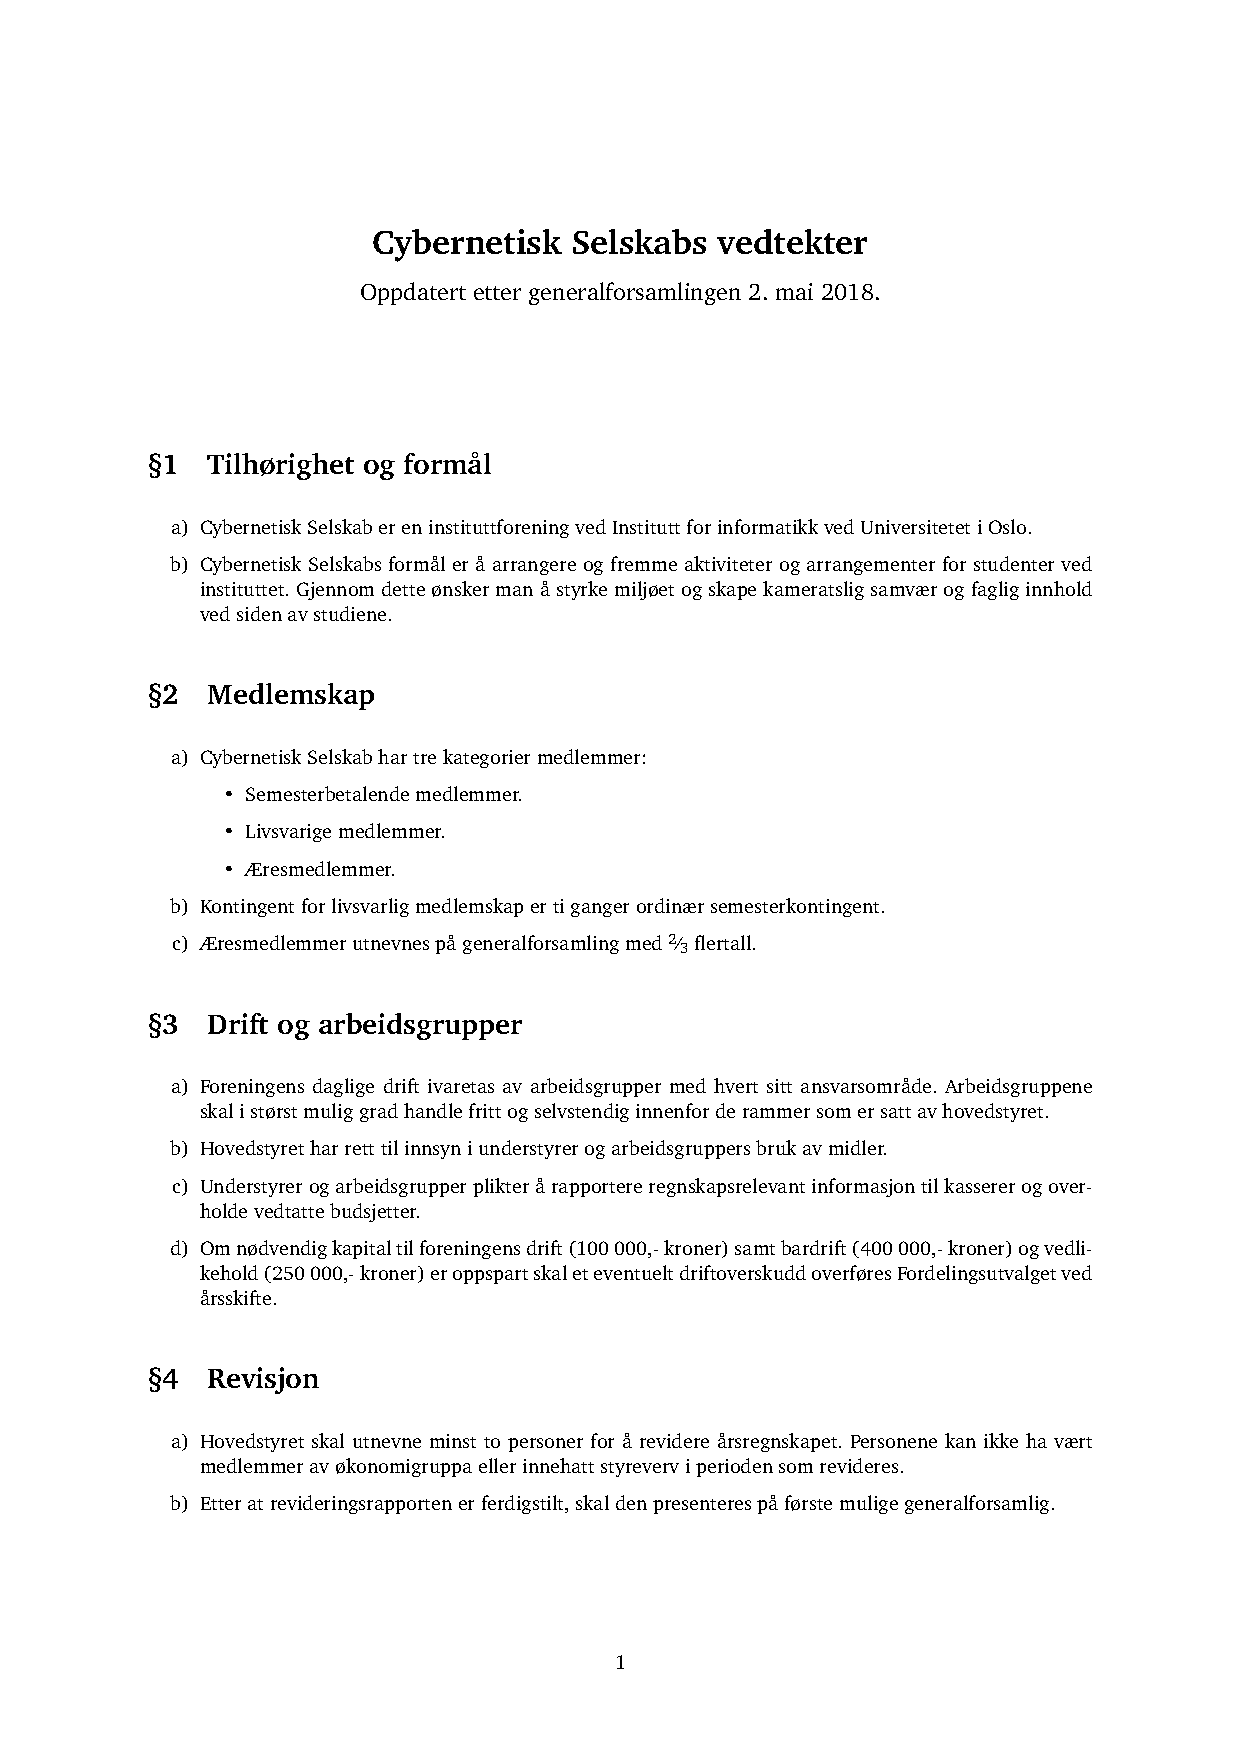
\includepdf[pages=-]{../vedtekter/vedtekter.pdf}

\end{document}
